\documentclass[a4paper,11pt,twoside]{report}
\usepackage{amsmath}
\usepackage{ascmac}
\usepackage[dvipdfmx]{graphicx}  % for EPS and PDF 
\usepackage{url}
\usepackage{fancyvrb}
\usepackage{makeidx}
\usepackage{float}
\usepackage[dvipdfmx]{color}
\usepackage{vruler}  %% if vertical ruler (line number) is needed
\usepackage[dvipdfm,bookmarkstype=toc,urlcolor=black,%
    linkcolor=black,citecolor=black,bookmarks=false]{hyperref}
\setcounter{secnumdepth}{4}
\setcounter{tocdepth}{3}
\setcounter{totalnumber}{6}
\usepackage{fancyhdr}

\let\olditemize\itemize
\renewcommand{\itemize}{
   \olditemize
   \setlength{\itemsep}{8pt}
   \setlength{\parskip}{0pt}
   \setlength{\parsep}{0pt}
}

\parindent = 0pt
\hoffset=0cm
\oddsidemargin=0cm
\evensidemargin=0cm
\textwidth=16cm
\topmargin=-1cm
\voffset=0cm
\textheight=24cm

\def\progenv{\baselineskip=10pt\tt\progspecial{`}\parindent=0.3cm}
\def\shellenv{\baselineskip=10pt\tt\progspecial{`}\parindent=0.3cm\nolineno}

\renewcommand{\topfraction}{.99}
\renewcommand{\bottomfraction}{.99}

\def\openb{{\it [}}
\def\closeb{{\it ]}}
\def\XMP{XcalableMP}
\def\XACC{XcalableACC}
\def\OACC{OpenACC}
\def\OMP{OpenMP}
\def\XMPF{XcalableMP Fortran}
\def\XMPC{XcalableMP C}
\def\XACCF{XcalableACC Fortran}
\def\XACCC{XcalableACC C}
\def\Syntax#1{\index{Syntax!#1@{\tt #1}}}
\def\Example#1{\index{Example!#1@{\tt #1}}}
%
\def\phrule{\vspace{0.2cm}\hrule\vspace{0.05cm}\hrule}
\def\qhrule{\vspace{0.2cm}\hrule}
\def\dhrule{\hrule\vspace{0.05cm}\hrule}
\def\bsquare{\rule[-2pt]{5pt}{10pt}}
%
\newenvironment{mytable}[3]{\begin{table}[ht]\caption{#1}\label{#2}\vspace*{-0.3cm}\begin{center}\begin{tabular}{#3}}{\end{tabular}\end{center}\end{table}}
\newenvironment{myfigure}{\begin{figure}[ht]\begin{center}}{\end{center}\end{figure}}
%
\DefineVerbatimEnvironment{XACCFexampleL}{Verbatim}{numbers=left,numbersep=3pt,stepnumber=5,frame=single,label=\XACCF}
\DefineVerbatimEnvironment{XACCCexampleR}{Verbatim}{numbers=right,numbersep=3pt,stepnumber=5,frame=single,label=\XACCC}
\DefineVerbatimEnvironment{XACCCexampleL}{Verbatim}{numbers=left,numbersep=3pt,stepnumber=5,frame=single,label=\XACCC}
%

\title{{\Huge XcalableACC}\\
$\langle${\it ex-scalable-a-c-c}$\rangle$\\
Language Specification\\
\vspace{2cm}
Version 1.0\\}
\author{
\Large RIKEN AICS and University of Tsukuba\\
}
\date{\vspace{4cm}\Large June 2017}

\makeindex

\begin{document}
\maketitle

Copyright \copyright 2017 Programming Environment Research Team of RIKEN AICS
and High Performance Computing System Laboratory of University of Tsukuba.
%Copyright \copyright 2016-2017 {\XMP} Specification Working Group.
%Permission to copy without fee all or part of this material is granted,
%provided the {\XMP} Specification Working Group copyright notice and the
%title of this document appear. Notice is given that copying is by permission
%of {\XMP} Specification Working Group.

\clearpage
%\setvruler[][][][3][0][1.2\textwidth]
\section*{History}

\paragraph*{Version 1.0: June 26, 2017}
First release.

\cleardoublepage

\pagenumbering{roman}
\tableofcontents

\newpage
\mbox{}\newpage

\pagestyle{fancy}
\fancyhead{} % clear all header fields
\fancyhead[RE]{\leftmark}
\fancyhead[LO]{\rightmark}
\fancyhead[LE,RO]{\thepage}
\fancyfoot{} % clear all footer fields
\renewcommand{\headrulewidth}{0pt}
\renewcommand{\footrulewidth}{0pt}

\chapter{Introduction}\label{chap:intro}
\pagenumbering{arabic}
\setcounter{page}{1}
This document defines the specification of {\XACC} which is an extension of {\XMP} version 1.3\cite{xmp} and {\OACC} version 2.5\cite{openacc}.
{\XACC} provides a parallel programming model for accelerated clusters
which are distributed memory systems equipped with accelerators.
In this document,
terminologies of {\XMP} and {\OACC} are indicated by {\bf bold font}.
For details, refer to each specification\cite{xmp,openacc}.

\section{Hardware Model}
The target of {\XACC} is an accelerated cluster,
a hardware model of which is shown in Fig. \ref{fig:hardware}.

\begin{myfigure}
  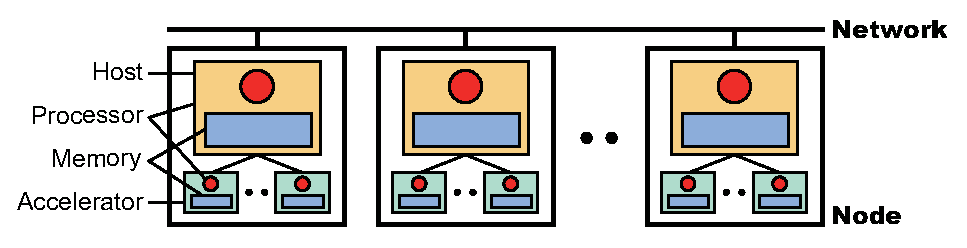
\includegraphics[scale=0.9,clip]{figs/hardware.eps}
  \caption{Hardware Model}\label{fig:hardware}
\end{myfigure}

An execution unit is called {\bf node} as with {\XMP}.
Each {\bf node} consists of a single host and multiple accelerators (such as GPUs and Intel MICs).
Each host has a processor, which may have several cores, and own local memory.
Each accelerator also has them.
Each {\bf node} is connected with each other via network.
Each {\bf node} can access its local memories directly and remote memories,
that is, the memories of another {\bf node} indirectly.
In a host,
the accelerator memory may be physically and/or virtually separate from the host memory as with the memory model of {\OACC}.
Thus,
a host may not be able to read or write the accelerator memory directly.

\section{Programming Model}
{\XACC} is a directive-based language extension based on Fortran 90 and ISO C90 (ANSI C90).
To develop applications on accelerated clusters with ease,
{\XACC} extends {\XACC} and {\OACC} independently as follow:
(1) {\XMP} extensions are to facilitate cooperation between {\XMP} and {\OACC} directives.
(2) {\OACC} extensions are to deal with multiple accelerators.

\subsection{{\XMP} Extensions}
In a program using the {\XMP} extensions,
{\XMP}, {\OACC}, and {\XACC} directives are used.
Fig. \ref{fig:concept} shows a concept of the {\XMP} extensions.

\begin{myfigure}
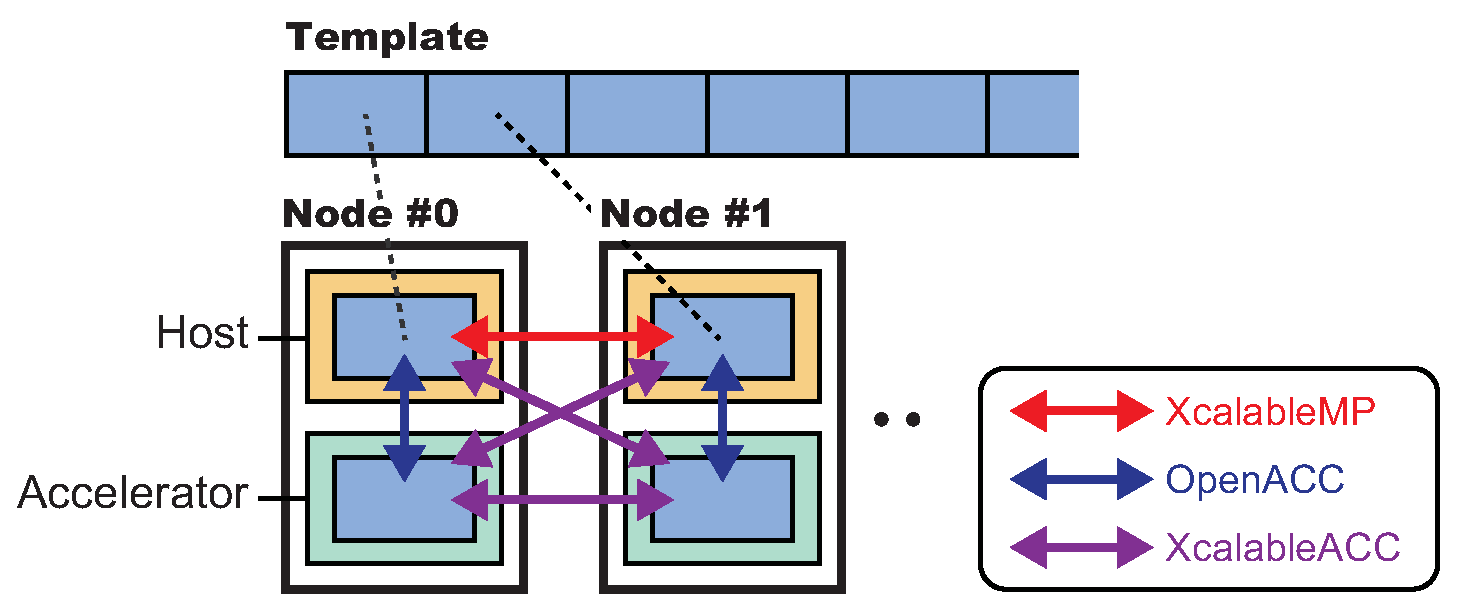
\includegraphics[scale=0.5,clip]{figs/concept.eps}
  \caption{Concept of {\XMP} Extensions}\label{fig:concept}
\end{myfigure}

{\XMP} directives define a {\bf template} and a {\bf node set}.
The {\bf template} represents a global index space, which is distributed onto the {\bf node set}.
Moreover, {\XMP} directives declare {\bf distributed arrays},
parallelize loop statements and transfer data among host memories according to the distributed {\bf template}.
{\OACC} directives transfer the {\bf distributed arrays} between host memory and accelerator memory on the same {\bf node}
and execute the loop statements parallelized by {\XMP} on accelerators in parallel.
{\XACC} directives, which are {\XMP} communication directives with an {\tt acc} clause, 
transfer data among accelerator memories and between accelerator memory and host memory on different {\bf nodes}.
Moreover, 
{\bf coarray} features also transfer data on different nodes.

%The {\XMP} extension is defined to develop parallel applications with keeping the sequential code image.
Note that 
the {\XMP} extensions are not a simple combination of {\XMP} and {\OACC}.
For example, 
if you represent communication of {\bf distributed array} among accelerators shown in Fig. \ref{fig:concept} by the combination of {\XMP} and {\OACC},
you need to specify explicitly communication between host and accelerator by {\OACC} and that between hosts by {\XMP}.
Moreover,
you need to calculate manually indices of the {\bf distributed array} owned by each {\bf node}.
By contrast,
{\XACC} directives can represent such communication among accelerators directly using global indices.

\subsection{{\OACC} Extensions}

\section{Execution Model}
The execution model of {\XACC} is a combination of those of {\XMP} and {\OACC}.
While the execution model of a host CPU programming is based on that of {\XMP},
that of an accelerator programming is based on that of {\OACC}.
Unless otherwise specified,
each {\bf node} behaves exactly as specified in the {\XMP} specification\cite{xmp} or the {\OACC} specification\cite{openacc}.
%For details, refer to each specification\cite{xmp,openacc}.

An {\XACC} program execution is based on the SPMD model, 
where each {\bf node} starts execution from the same main routine and keeps executing the same code independently (i.e. asynchronously), 
which is referred to as the replicated execution
until it encounters an {\XMP} construct or an {\XMP}-extension construct.
In particular,
the {\XMP}-extension construct may allocate, deallocate, or transfer data on accelerators.
An {\OACC} construct or an {\OACC}-extension construct may define {\bf parallel regions}, such as work-sharing loops, 
and offloads it to accelerators under control of the host.

When a {\bf node} encounters a loop construct 
targeted by a combination of {\XMP} {\tt loop} and {\OACC} {\tt loop} directives,
it executes the loop construct in parallel with other {\bf accelerators},
so that each iteration of the loop construct is independently executed by the {\bf accelerator}
where a specified data element resides.

When a {\bf node} encounters a {\XACC} synchronization or a {\XACC} communication directive,
synchronization or communication occurs between it and other accelerators.
That is, such {\bf global constructs} are performed collectively by the {\bf current executing nodes}.
Note that neither synchronizations nor communications occur without these constructs specified.

\section{Data Model}
There are two classes of data in {\XACC}: {\bf global data} and {\bf local data} as with {\XMP}. 
Data declared in an {\XACC} program are local by default.
Both {\bf global data} and {\bf local data} can exist on host memory and accelerator memory.
About the data models of host memory and accelerator memory, refer to the OpenACC specification\cite{openacc}.

{\bf Global data} are ones that are distributed onto the {\bf executing node set} by the {\tt align} directive.
Each fragment of a {\bf global data} is allocated in host memory of a {\bf node} in the {\bf executing node set}.
{\OACC} directives can transfer the fragment from host memory to accelerator memory.

{\bf Local data} are all of the ones that are not global.
They are replicated in the local memory of each of the {\bf executing nodes}.

A {\bf node} can access directly only {\bf local data} and sections of {\bf global data} that are allocated in its local memory.
To access data in remote memory, 
explicit communication must be specified in such ways as the global communication constructs and the {\bf coarray} assignments.

Particularly in {\XACCF}, 
for common blocks that include any global variables, 
the ways how the storage sequence of them is defined and how the storage association of them is resolved are implementation-dependent.

\section{Directive Format}
This section describes the syntax and behavior of {\XMP} and {\OACC} directives in {\XACC}.
In this document, 
the following notation is used to describe the directives.

\vspace{0.5cm}%
\begin{tabular}{ll}
{\tt xxx} & {\tt type-face} characters are used to indicate literal type characters. \\
{\it xxx...} & If the line is followed by ``...'', then xxx can be repeated. \\
{\it [xxx]} & {\it xxx} is optional. \\
{\bsquare} & The syntax rule continues. \\
\verb![F]! & The following lines are effective only in {\XACCF}. \\
\verb![C]! & The following lines are effective only in {\XACCC}. \\
\end{tabular}
\vspace{0.5cm}%

In {\XACCF}, 
{\XMP} and {\OACC} directives are specified using special comments that are identified by unique sentinels {\tt\verb|!$xmp|} and {\tt\verb|!$acc|} respectively.
the directives follow the rules for comment lines of either the Fortran free or fixed source form,
depending on the source form of the surrounding program unit\footnote{Consequently, the rules of comment lines that an
{\XMP} directive follows is the same as the ones that an {\OMP} directive follows.}.
The directives are case-insensitive.

\vspace{0.5cm}
\Syntax{directive}
\begin{tabular}{ll}
\verb![F]! & \verb|!$xmp| {\it directive-name clause} \\
\verb![F]! & \verb|!$acc| {\it directive-name clause} \\
\end{tabular}
\vspace{0.5cm}

In {\XACC}, 
{\XMP} and {\OACC} directives are specified using the \verb|#pragma| mechanism provided by the C standards.
the directives are case-sensitive.

\vspace{0.5cm}
\Syntax{directive}
\begin{tabular}{ll}
\verb![C]! & \verb|#pragma xmp| {\it directive-name clause} \\
\verb![C]! & \verb|#pragma acc| {\it directive-name clause} \\
\end{tabular}
\vspace{0.5cm}

%Directives are classified as {\bf declarative directives} and {\bf executable directives}\cite{xmp}.
%
%The {\bf declarative directives} are {\tt nodes}, {\tt template}, {\tt distribute}, {\tt align},
%{\tt shadow}, {\tt coarray}, {\tt declare}, and {\tt routine} directives.
%
%The {\bf executable directives} are {\tt template\_fix}, {\tt task}, {\tt tasks}, {\XMP} {\tt loop}, 
%{\tt array}, {\tt reflect}, {\tt reflect\_init}, {\tt reflect\_do}, {\tt gmove}, {\tt barrier}, 
%{\tt reduction}, {\tt bcast}, {\tt wait\_async},
%{\tt parallel}, {\tt kernels}, {\tt data}, {\tt host\_data}, {\OACC} {\tt loop},
%{\tt cache}, {\tt atomic}, {\tt init}, {\tt shutdown}, {\tt set}, {\tt update}, 
%{\tt wait}, {\tt enter\_data}, and {\tt exit\_data} directives.
%An {\bf executable directive} and its associated user code make up an {\XACC} construct, 
%as in the following format:
%
%\vspace{0.5cm}
%\begin{tabular}{ll}
%\verb![F]! & \verb|!$xmp| {\it directive-name clause} ...\\
% & \hspace{0.5cm} {\it structured-block} \\
%\verb![F]! & \verb|!$acc| {\it directive-name clause} ...\\
% & \hspace{0.5cm} {\it structured-block} \\
%\end{tabular}
%
%\vspace{0.3cm}
%
%\begin{tabular}{ll}
%\verb![C]! & \verb|#pragma xmp| {\it directive-name clause} ...\\
% & \hspace{0.5cm} {\it structured-block} \\
%\verb![C]! & \verb|#pragma acc| {\it directive-name clause} ...\\
% & \hspace{0.5cm} {\it structured-block} \\
%\end{tabular}
%\vspace{0.5cm}

\section{Organization of This Document}
The remainder of this document is structured as follows:

\begin{itemize}
 \item Chapter 2: {\XMP} Extensions
 \item Chapter 3: {\OACC} Extensions
\end{itemize}
 \cleardoublepage
\chapter{{\XMP} Extension}\label{chap:xmp-ex}
This chapter defines a behavior of mixing {\XMP} and {\OACC}.
Note that the existing {\OACC} is not extended in the {\XMP} extension.
The {\XMP} extension can represent 
(1) parallelization with keeping sequential code image using a combination of {\XMP} and {\OACC},
and
(2) communication among accelerator memories and between accelerator memory and host memory on different {\tt nodes}
using {\XACC} directives or {\tt coarray} features.

\section{Combination of {\XMP} and {\OACC}}
\subsection{{\OACC} Directives on Data}
\subsubsection*{Description}
When {\tt distributed arrays} appear in {\OACC} constructs,
global indices in {\tt distributed arrays} are used.
%Thus,
%an {\XACC} compiler automatically translates the global indices in the {\OACC} constructs to the appropriate local indices.
The {\tt distributed arrays} may appear in the {\OACC} {\bf update}, {\bf enter data}, {\bf exit data}, 
{\bf host\_data}, {\bf cache}, and {\bf declare} directives,
and the {\bf data} clause accompanied by some of 
{\bf deviceptr}, {\bf present}, {\bf copy}, {\bf copyin}, 
{\bf copyout}, {\bf create}, and {\bf delete} clauses.
Data transfer of {\tt distributed array} by {\OACC} is performed on only {\tt nodes} which have elements specified by the global indices.

\subsubsection*{Example}
\begin{myfigure}
\begin{minipage}{0.45\hsize}
\begin{center}
\begin{XACCFexampleL}
integer :: a(N), b(N)
!$xmp template t(N)
!$xmp nodes p(*)
!$xmp distribute t(block) onto p
!$xmp align a(i) with t(i)
!$xmp align b(i) with t(i)
...
!$acc enter data copyin(a(1:k))
!$acc data copy(b)
...
\end{XACCFexampleL}
\end{center}
\end{minipage}
%
\begin{minipage}{0.53\hsize}
\begin{center}
\begin{XACCCexampleR}
int a[N], b[N];
#pragma xmp template t[N]
#pragma xmp nodes p[*]
#pragma xmp distribute t[block] onto p
#pragma xmp align a[i] with t[i]
#pragma xmp align b[i] with t[i]
...
#pragma acc enter data copyin(a[0:k])
#pragma acc data copy(b)
{ ...
\end{XACCCexampleR}
\end{center}
\end{minipage}
\caption{Code example in {\XMP} extension with {\OACC} {\bf enter\_data} directive}\label{code:ex-oacc-data}
\end{myfigure}

In lines 2-6,
{\XMP} directives declare the {\tt distributed arrays} {\it a} and {\it b}.
In line 8,
the {\OACC} {\bf enter data} directive transfers the certain range of the {\tt distributed array} {\it a} from host memory to accelerator memory.
Note that the range is represented by global indices.
In line 9,
the {\OACC} {\bf data} directive transfers the whole {\tt distributed array} {\it b} from host memory to accelerator memory.

\subsection{{\OACC} Loop Construct}
\subsubsection*{Description}
In order to perform a loop statement on accelerators in {\tt nodes} in parallel,
{\XMP} {\bf loop} directive and {\OACC} {\bf loop} directive are used.
While
{\XMP} {\bf loop} directive performs a loop statement in {\tt nodes} in parallel,
{\OACC} {\bf loop} directive also performs the loop statement parallelized by the {\XMP} {\bf loop} directive 
on accelerators in parallel.
For ease of writing,
the order of {\XMP} {\bf loop} directive and {\OACC} {\bf loop} directive does not matter.

\subsubsection*{Restriction}
\begin{itemize}
\item In {\OACC} {\tt compute region},
only {\XMP} {\bf loop} directive without {\bf reduction} clause can be inserted.
\item In {\OACC} {\tt compute region},
targeted loop condition (lower bound, upper bound, and step of the loop)
must remain unchanged.
\end{itemize}

\subsubsection*{Example}
\begin{myfigure}
\begin{minipage}{0.45\hsize}
\begin{center}
\begin{XACCFexampleL}
integer :: a(N), b(N), sum = 0
!$xmp template t(N)
!$xmp nodes p(*)
!$xmp distribute t(block) onto p
!$xmp align a(i) with t(i)
!$xmp align b(i) with t(i)
...
!$acc parallel loop copy(a, b)
!$xmp loop on t(i)
do i=0, N
  b(i) = a(i)
end do
!$acc end parallel
\end{XACCFexampleL}
\end{center}
\end{minipage}
%
\begin{minipage}{0.53\hsize}
\begin{center}
\begin{XACCCexampleR}
int a[N], b[N], sum = 0;
#pragma xmp template t[N]
#pragma xmp nodes p[*]
#pragma xmp distribute t[block] onto p
#pragma xmp align a[i] with t[i]
#pragma xmp align b[i] with t[i]
...
#pragma acc parallel loop copy(a, b)
#pragma xmp loop on t[i]
for(int i=0;i<N;i++){
  b[i] = a[i];
}

\end{XACCCexampleR}
\end{center}
\end{minipage}
\caption{Code example in {\XMP} extension with {\OACC} loop construct}\label{code:ex-oacc-loop}
\end{myfigure}

In lines 2-6,
{\XMP} directives declare {\tt distributed arrays} {\it a} and {\it b}.
In line 8,
{\OACC} {\bf parallel} directive with {\bf data} clause transfers the {\tt distributed arrays} {\it a} and {\it b} from host memory to accelerator memory.
Moreover,
in lines 8-9,
{\OACC} {\bf parallel} directive and {\XMP} {\bf loop} directive perform the next loop statement on accelerators in {\tt nodes} in parallel.

\section{Communication on Accelerated Clusters}
\subsection{{\XACC} Directives}
{\XACC} directives are extensions of {\XMP} {\bf reflect}, {\bf gmove}, 
{\bf barrier}, {\bf reduction}, {\bf bcast}, and {\bf wait\_async} directives in {\XMP} global-view memory model.
When adding an {\bf acc} clause to the above {\XMP} directives,
data stored on accelerator memory are transferred.
Note that while XcalableACC {\bf gmove} directive described in Section \ref{sec:reflect} 
and {\tt coarray} features described in Section \ref{sec:coarray} can occur communication both among accelerator memories and between accelerator memory and host memory on different {\tt nodes},
other directives can occur communication only among accelerator memories.

This section describes only the extended parts of {\XACC} directives from {\XMP} directives. 
For other information, refer to the {\XMP} specification\cite{xmp}.

\subsubsection{reflect Construct}\label{sec:reflect}
\subsubsection*{Synopsis}
The {\bf reflect} construct assigns the value of a
reflection source to the corresponding shadow object.

\subsubsection*{Syntax}
\begin{tabular}{ll}
 \verb![F]! & \verb|!$xmp| {\tt reflect} \verb|(| {\it array-name}
 {\openb}, {\it array-name}{\closeb}... \verb|)| {\bsquare} \\
 &\hspace{0.1cm} {\bsquare} {\openb}{\tt width (} {\it reflect-width}
     {\openb}, {\it reflect-width}{\closeb}... {\tt )}{\closeb}
     {\openb}{\tt orthogonal}{\closeb}
     {\openb}{\tt async (} {\it async-id} {\tt )}{\closeb} {\openb}{\tt acc}{\closeb}\\
\verb![C]! & \verb|#pragma xmp| {\tt reflect} \verb|(| {\it array-name}
     {\openb}, {\it array-name}{\closeb}... \verb|)| {\bsquare} \\
 &\hspace{0.1cm} {\bsquare} {\openb}{\tt width (} {\it reflect-width}
     {\openb}, {\it reflect-width}{\closeb}... {\tt )}{\closeb}
     {\openb}{\tt orthogonal}{\closeb}
     {\openb}{\tt async (} {\it async-id} {\tt )}{\closeb} {\openb}{\tt acc}{\closeb}\\
\end{tabular}

\vspace{1em}
where {\it reflect-width} must be one of:
\vspace{1em}

\begin{tabular}{ll}
 \hspace{0.5cm} & {\openb}{\tt /periodic/}{\closeb} {\it int-expr} \\
                & {\openb}{\tt /periodic/}{\closeb} {\it int-expr} : {\it int-expr}
\end{tabular}

\subsubsection*{Description}
When the {\bf acc} clause is specified,
the {\bf reflect} construct updates each of the shadow object of the
array specified by {\it array-name} on accelerator memory with the value of its corresponding
reflection source.

\subsubsection*{Restriction}
\begin{itemize}
 \item When the {\bf acc} clause is specified,
   the arrays specified by the sequence of {\it array-name}'s must be allocated on accelerator memory.
 \item This construct must not appear in {\OACC} {\tt compute region}.
\end{itemize}

\subsubsection*{Example}
\begin{myfigure}
\begin{minipage}{0.45\hsize}
\begin{center}
\begin{XACCFexampleL}
integer :: a(N)
!$xmp template t(N)
!$xmp nodes p(*)
!$xmp distribute t(block) onto p
!$xmp align a(i) with t(i)
!$xmp shadow a(1)
...
!$acc enter data copyin(a)
!$xmp reflect (a) acc
\end{XACCFexampleL}
\end{center}
\end{minipage}
%
\begin{minipage}{0.53\hsize}
\begin{center}
\begin{XACCCexampleR}
int a[N];
#pragma xmp template t[N]
#pragma xmp nodes p[*]
#pragma xmp distribute t[block] onto p
#pragma xmp align a[i] with t[i]
#pragma xmp shadow a[1]
...
#pragma acc enter data copyin(a)
#pragma xmp reflect (a) acc
\end{XACCCexampleR}
\end{center}
\end{minipage}
\caption{Code example in {\XACC} {\bf reflect} construct}\label{code:reflect}
\end{myfigure}

In lines 2-5,
{\XMP} directives declare {\tt distributed array} {\it a}.
In line 6, 
{\XMP} {\bf shadow} directive allocates shadow areas of the {\tt distributed array} {\it a}.
In line 8,
{\OACC} {\bf enter data} directive transfers the {\tt distributed array} {\it a} with the shadow areas from host memory to accelerator memory.
In line 9,
{\XACC} {\bf reflect} directive updates the shadow areas of the {\tt distributed array} {\it a} on accelerator memory between neighboring {\tt nodes}.

\subsubsection{gmove Construct}\label{sec:gmove}
\subsubsection*{Synopsis}
The {\tt \Directive{gmove}} construct allows an assignment statement,
which may cause communication, to be executed possibly in parallel by
the executing {\tt nodes}.

\subsubsection*{Syntax}
\begin{tabular}{ll}
\verb![F]! & \verb|!$xmp| {\tt gmove} {\openb}{\tt in} $\vert$ {\tt
 out}{\closeb} {\openb}{\tt async (} {\it async-id} {\tt )}{\closeb} {\openb}{\tt acc}{\openb}({\it variable}){\closeb}{\closeb}\\
\verb![C]! & \verb|#pragma xmp| {\tt gmove} {\openb}{\tt in} $\vert$ {\tt
 out}{\closeb} {\openb}{\tt async (} {\it async-id} {\tt )}{\closeb} {\openb}{\tt acc}{\openb}({\it variable}){\closeb}{\closeb}\\
\end{tabular}

\subsubsection*{Description}
\begin{itemize}
 \item When the {\bf acc} clause is specified and the variable is not specified by {\it variable} in the parenthesis,
variables of both sides in the assignment statement on accelerator memory are targeted.
 \item When the {\bf acc} clause is specified and the variable is specified by {\it variable} in the parenthesis,
the specified variable on accelerator memory is targeted, 
and the unspecified variable on host memory is targeted.
\end{itemize}

\subsubsection*{Restriction}
\begin{itemize}
 \item The variables targeted on accelerator memory must be allocated on accelerator memory.
 \item This construct must not appear in {\OACC} {\tt compute region}.
\end{itemize}

\subsubsection*{Example}
\begin{myfigure}
\begin{minipage}{0.45\hsize}
\begin{center}
\begin{XACCFexampleL}
integer :: a(N), b(N)
!$xmp template t(N)
!$xmp nodes p(*)
!$xmp distribute t(block) onto p
!$xmp align a(i) with t(i)
!$xmp align b(i) with t(i)
...
!$acc enter data copyin(a, b)
!$xmp gmove acc
  a(:) = b(:)

!$xmp gmove acc(b)
  a(:) = b(:)
\end{XACCFexampleL}
\end{center}
\end{minipage}
%
\begin{minipage}{0.53\hsize}
\begin{center}
\begin{XACCCexampleR}
int a[N], b[N];
#pragma xmp template t[N]
#pragma xmp nodes p[*]
#pragma xmp distribute t[block] onto p
#pragma xmp align a[i] with t[i]
#pragma xmp align b[i] with t[i]
...
#pragma acc enter data copyin(a, b)
#pragma xmp gmove acc
  a[:] = b[:];

#pragma xmp gmove acc(b)
  a[:] = b[:];
\end{XACCCexampleR}
\end{center}
\end{minipage}
\caption{Code example in {\XACC} {\bf gmove} construct}\label{code:gmove}
\end{myfigure}

In lines 2-6,
{\XMP} directives declare {\tt distributed arrays} {\it a} and {\it b}.
In line 8,
{\OACC} {\bf enter data} directive transfers the {\tt distributed arrays} {\it a} and {\it b} from host memory to accelerator memory.
In lines 9-10,
{\XACC} {\bf gmove} construct copies the whole {\tt distributed array} {\it b} to
that of the {\tt distributed array} {\it a} on accelerator memories.
In lines 12-13,
{\XACC} {\bf gmove} construct copies the whole {\tt distributed array} {\it b} on accelerator memory to
that of the {\tt distributed array} {\it a} on host memory.

\subsubsection{barrier Construct}\label{sec:barrier}
\subsubsection*{Synopsis}
The {\bf barrier} construct specifies an explicit barrier
at the point at which the construct appears.

\subsubsection*{Syntax}
\begin{tabular}{ll}
\verb![F]! & \verb|!$xmp| {\tt barrier} {\openb}{\tt on} {\it nodes-ref}
 $\vert${\it template-ref}{\closeb} {\openb}{\tt acc}{\closeb}\\
\verb![C]! & \verb|#pragma xmp| {\tt barrier} {\openb}{\tt on} {\it
     nodes-ref} $\vert$ {\it template-ref}{\closeb} {\openb}{\tt acc}{\closeb}\\
\end{tabular}

\subsubsection*{Description}
\begin{itemize}
 \item When the {\bf acc} clause is specified,
the barrier construct blocks until all outgoing asynchronous operations on accelerators are completed.
 \item When the {\bf acc} clause is not specified,
the barrier construct does not guarantee that an outgoing asynchronous operation on accelerator is completed.
\end{itemize}

\subsubsection*{Example}
\begin{myfigure}
\begin{minipage}{0.45\hsize}
\begin{center}
\begin{XACCFexampleL}
!$xmp nodes p(*)
...
!$xmp barrier acc
\end{XACCFexampleL}
\end{center}
\end{minipage}
%
\begin{minipage}{0.53\hsize}
\begin{center}
\begin{XACCCexampleR}
#pragma xmp nodes p[*]
...
#pragma xmp barrier acc
\end{XACCCexampleR}
\end{center}
\end{minipage}
\caption{Code example in {\XACC} {\bf barrier} construct}\label{code:barrier}
\end{myfigure}

In line 1,
{\XMP} {\bf nodes} directive defines {\tt node set} {\it p}.
In line 3,
{\XACC} {\bf barrier} directive performs a barrier operation for accelerators on all {\tt node}.

\subsubsection{reduction Construct}\label{sec:reduction}
\subsubsection*{Synopsis}
The {\bf reduction} construct performs a reduction operation among {\tt nodes}.

\subsubsection*{Syntax}
\Syntax{reduction}

\begin{tabular}{ll}
\verb![F]! & \verb|!$xmp| {\tt reduction (} {\it reduction-kind} {\it
  :} {\it variable} {\openb}, {\it variable} {\closeb}... {\tt )}
 {\bsquare} \\
 & \hspace{5cm} {\bsquare} {\openb}{\tt on} {\it node-ref} $\vert$ {\it
     template-ref}{\closeb} {\openb}{\tt async (} {\it async-id} {\tt )}{\closeb} {\openb}{\tt acc}{\closeb}\\
\end{tabular}

\vspace{0.5cm}
where {\it reduction-kind} is one of:

\begin{tabular}{ll}
 \hspace{0.5cm} & {\tt +} \\
 & {\tt *} \\
% & {\tt -} \\
 & {\tt .and.} \\
 & {\tt .or.} \\
 & {\tt .eqv.} \\
 & {\tt .neqv.} \\
 & {\tt max} \\
 & {\tt min} \\
 & {\tt iand} \\
 & {\tt ior} \\
 & {\tt ieor} \\
\end{tabular}

\vspace{0.5cm}

\begin{tabular}{ll}
 \hspace{-\parindent}
 \verb![C]! & \verb|#pragma xmp| {\tt reduction (} {\it reduction-kind} {\it
  :} {\it variable} {\openb}, {\it variable} {\closeb}... {\tt )}
 {\bsquare} \\
 & \hspace{5cm} {\bsquare} {\openb}{\tt on} {\it node-ref} $\vert$ {\it
     template-ref}{\closeb} {\openb}{\tt async (} {\it async-id} {\tt )}{\closeb} {\openb}{\tt acc}{\closeb} \\
\end{tabular}
\vspace{0.5cm}

where {\it reduction-kind} is one of:

\begin{tabular}{ll}
 \hspace{0.5cm} & {\tt +} \\
 & {\tt *} \\
% & {\tt -} \\
 & {\verb|&|} \\
 & {\tt |} \\
 & {\verb|^|} \\
 & {\verb|&&|} \\
 & {\tt ||} \\
 & {\tt max} \\
 & {\tt min} \\
\end{tabular}

\subsubsection*{Description}
When the {\bf acc} clause is specified,
the {\tt reduction} construct performs a type of
reduction operation specified by {\it reduction-kind} for the specified
local variables among the accelerators and 
sets the reduction results to the variables on each of the accelerators.

\subsubsection*{Restriction}
\begin{itemize}
 \item When the {\bf acc} clause is specified,
   the variables specified by the sequence of {\it variable}'s must be allocated on accelerator memory.
 \item This construct must not appear in {\OACC} {\tt compute region}.
\end{itemize}

\subsubsection*{Example}
\begin{myfigure}
\begin{minipage}{0.45\hsize}
\begin{center}
\begin{XACCFexampleL}
integer :: a
!$xmp nodes p(*)
...
!$acc enter data copyin(a)
!$xmp reduction(+:a) acc
\end{XACCFexampleL}
\end{center}
\end{minipage}
%
\begin{minipage}{0.53\hsize}
\begin{center}
\begin{XACCCexampleR}
int a;
#pragma xmp nodes p[*]
...
#pragma acc enter data copyin(a)
#pragma xmp reduction(+:a) acc
\end{XACCCexampleR}
\end{center}
\end{minipage}
\caption{Code example in {\XACC} {\bf reduction} construct}\label{code:reduction}
\end{myfigure}

In line 2,
{\XMP} {\bf nodes} directive defines {\tt node set} {\it p}.
In line 4,
{\OACC} {\bf enter data} directive transfers the local variable {\it a} from host memory to accelerator memory.
In line 5,
{\XACC} {\bf reduction} directive calculates a total value of the variable {\it a} stored on each accelerator
memory in each {\tt node}.

\subsubsection{bcast Construct}\label{sec:bcast}
\subsubsection*{Synopsis}
The {\bf bcast} construct performs broadcast communication from a specified {\tt node}.

\subsubsection*{Syntax}

\begin{tabular}{ll}
 \verb![F]! & \verb|!$xmp| {\tt bcast} \verb|(| {\it variable}
 {\openb}, {\it variable}{\closeb}... \verb|)|
 {\openb}{\tt from} {\it nodes-ref} $\vert$ {\it template-ref}{\closeb}
 {\bsquare} \\
 & \hspace{4.8cm} {\bsquare} {\openb}{\tt on} {\it nodes-ref}{\closeb}
     $\vert$ {\it template-ref}{\closeb}
     {\openb}{\tt async (} {\it async-id} {\tt )}{\closeb} {\openb}{\tt acc}{\closeb}\\

 \verb![C]! & \verb|#pragma xmp| {\tt bcast} \verb|(| {\it variable}
 {\openb}, {\it variable}{\closeb}... \verb|)|
 {\openb}{\tt from} {\it nodes-ref}  $\vert$ {\it
     template-ref}{\closeb} {\bsquare} \\
 & \hspace{4.8cm} {\bsquare} {\openb}{\tt on} {\it nodes-ref} $\vert$ {\it
     template-ref}{\closeb}
 {\openb}{\tt async (} {\it async-id} {\tt )}{\closeb} {\openb}{\tt acc}{\closeb}\\
\end{tabular}

\subsubsection*{Description}
When the {\bf acc} clause is specified, 
the values of the variables specified by the sequence of {\it variable}'s on accelerator memory
(called {\tt broadcast variables}) are broadcasted
from the {\tt node} specified by the {\tt from} clause (called the
{\tt source node}) to each of the {\tt nodes} in the {\tt node set} specified
by the {\tt on} clause. After executing this construct,
the values of the {\tt broadcast variables} become the same as those in the {\tt source node}.

\subsubsection*{Restriction}
\begin{itemize}
 \item When the {\bf acc} clause is specified,
   the variables specified by the sequence of {\it variable}'s must be allocated on accelerator memory.
 \item This construct must not appear in {\OACC} {\tt compute region}.
\end{itemize}

\subsubsection*{Example}
\begin{myfigure}
\begin{minipage}{0.45\hsize}
\begin{center}
\begin{XACCFexampleL}
integer :: a
!$xmp nodes p(*)
...
!$acc enter data copyin(a)
!$xmp bcast(a) acc
\end{XACCFexampleL}
\end{center}
\end{minipage}
%
\begin{minipage}{0.53\hsize}
\begin{center}
\begin{XACCCexampleR}
int a;
#pragma xmp nodes p[*]
...
#pragma acc enter data copyin(a)
#pragma xmp bcast(a) acc
\end{XACCCexampleR}
\end{center}
\end{minipage}
\caption{Code example in {\XACC} {\bf bcast} construct}\label{code:bcast}
\end{myfigure}

In line 2,
{\XMP} {\bf nodes} directive defines {\tt node set} {\it p}.
In line 4,
{\OACC} {\bf enter data} directive transfers the local variable {\it a} from host memory to accelerator memory.
In line 5,
{\XACC} {\bf bcast} directive broadcasts the variable {\it a} stored on accelerator memory to all {\it nodes}.

\subsubsection{wait\_async Construct}\label{sec:waitasync}
\subsubsection*{Synopsis}
The {\bf wait\_async} construct guarantees asynchronous
communications specified by {\it async-id} are complete.

\subsubsection*{Syntax}
\begin{tabular}{ll}
\verb![F]! & \verb|!$xmp| {\tt wait\_async ( {\it async-id} {\openb},
 {\it async-id} {\closeb}...)} {\openb}{\tt on} {\it nodes-ref} $\vert$
 {\it template-ref}{\closeb} {\openb}{\tt acc}{\closeb}\\
\verb![C]! & \verb|#pragma xmp| {\tt wait\_async ( {\it async-id} {\openb},
 {\it async-id} {\closeb}...)} {\openb}{\tt on} {\it nodes-ref} $\vert$
 {\it template-ref}{\closeb} {\bsquare} \\
& \hspace{13.5cm} {\bsquare} {\openb}{\tt acc}{\closeb}\\
\end{tabular}

\subsubsection*{Description}
When the {\bf acc} clause is specified,
the {\bf wait\_async} construct blocks and therefore
statements following it are not executed until all of the asynchronous
communications that are specified by {\it async-id}'s and issued on the accelerators in
{\tt node set} specified by the {\tt on} clause are complete.

\subsubsection*{Restriction}
This construct must not appear in {\OACC} {\tt compute region}.

\subsubsection*{Example}
\begin{myfigure}
\begin{minipage}{0.45\hsize}
\begin{center}
\begin{XACCFexampleL}
integer :: a
!$xmp nodes p(*)
...
!$acc enter data copyin(a)
!$xmp reduction(+:a) acc async(1)
...
!$xmp wait_async(1) acc
\end{XACCFexampleL}
\end{center}
\end{minipage}
%
\begin{minipage}{0.53\hsize}
\begin{center}
\begin{XACCCexampleR}
int a;
#pragma xmp nodes p[*]
...
#pragma acc enter data copyin(a)
#pragma xmp reduction(+:a) acc async(1)
...
#pragma xmp wait_async(1) acc
\end{XACCCexampleR}
\end{center}
\end{minipage}
\caption{Code example in {\XACC} {\bf wait\_async} construct}\label{code:waitasync}
\end{myfigure}

In line 2,
{\XMP} {\bf nodes} directive defines {\tt node set} {\it p}.
In line 4,
{\OACC} {\bf enter data} directive transfers the local variable {\it a} from host memory to accelerator memory.
In line 5,
{\XACC} {\bf reduction} directive performs asynchronously.
In line 7,
{\XACC} {\bf wait\_async} construct blocks until the asynchronous {\bf reduction} operation at line 5 is complete.

\subsection{Coarray Features} \label{sec:coarray}
\subsubsection*{Synopsis}
{\XACC} can perform one-sided communication (put/get operations) for data on accelerator memory using {\tt coarray} features,
which is based on {\XMP} local-view memory model.
A combination of {\tt coarray} syntax and {\OACC} {\bf host\_data} construct enables communication between accelerators.

\subsubsection*{Description}
If {\tt coarrays} appear in {\OACC} {\bf use\_device} clause of any {\OACC} enclosing {\bf host\_data} construct, 
communication targets data on the accelerator side. 
{\tt Coarray} operations on accelerators are synchronized using the same synchronization functions in {\XMP}.

\subsubsection*{Restriction}
\begin{itemize}
 \item Only {\OACC} {\bf declare} directive can declare a {\tt coarray} on accelerator memory.
   For example,
   {\OACC} {\bf enter data} and {\bf copy} directives cannot declare a {\tt coarray} on accelerator memory.
 \item The {\tt coarray} syntax must not appear in {\OACC} {\tt compute region}.
\end{itemize}

\subsubsection*{Example}
\begin{myfigure}
\begin{minipage}{0.45\hsize}
\begin{center}
\begin{XACCFexampleL}
integer :: a(N)[*]
integer :: b(N)
!$acc declare create(a, b)
...
if(this_image() == 1) then
!$acc host_data use_device(a, b)
  a(:)[2] = b(:)

!$acc host_data use_device(a)
  b(:) = a(:)[3]
end if
...
sync all
\end{XACCFexampleL}
\end{center}
\end{minipage}
%
\begin{minipage}{0.53\hsize}
\begin{center}
\begin{XACCCexampleR}
int a[N]:[*];
int b[N];
#pragma acc declare create(a, b)
...
if(xmp_node_num() == 1){
#pragma acc host_data use_device(a, b)
  a[:]:[2] = b[:];

#pragma acc host_data use_device(a)
  b[:] = a[:]:[3];
}
...
xmp_sync_all(NULL);
\end{XACCCexampleR}
\end{center}
\end{minipage}
\caption{Code example in {\XACC} coarray features}\label{code:coarray}
\end{myfigure}

In line 3,
{\OACC} {\bf declare} directive declares a {\tt coarray} {\it a} and a array {\it b} on accelerator memory.
In lines 6-7,
{\tt node} 1 performs put operation, where
the whole array {\it b} on accelerator memory in {\tt node} 1 is transferred to the {\tt coarray} {\it a} on accelerator memory in {\tt node} 2.
In lines 9-10,
{\tt node} 1 performs get operation, where
the whole {\tt coarray} {\it a} on accelerator memory in {\tt node} 3 is transferred to the array {\it b} on host memory in {\tt node} 1.
In line 13,
the {\bf sync all} statement in {\XACCF} or the {\bf xmp\_sync\_all} function in {\XACCC} synchronizes all {\tt nodes} and guarantees completion of ongoing coarray operations.

 \cleardoublepage
\chapter{{\OACC} Extensions}\label{chap:acc-ex}
This chapter defines an extension of {\OACC} in {\XACC}.
The extension can represent offload works to multiple-accelerators on each {\bf node}.

\section{Device Set Definition and Reference}
\subsection{devices Directive}\label{sec:devices}
\subsection*{Synopsis}
The {\bf devices} directive declares a set of devices.

\subsubsection*{Syntax}
\begin{tabular}{ll}
  \verb![F]! & \verb|!$acc| {\tt devices} {\it devices-decl} {\openb}, {\it devices-decl} {\closeb}...\\
  \verb![C]! & \verb|#pragma acc| {\tt devices} {\it devices-decl} {\openb}, {\it devices-decl} {\closeb}...
\end{tabular}

\vspace{1em}
where {\it device-decl} is one of:
\vspace{1em}

\begin{tabular}{lll}
  \hspace{0.5cm} & & {\it devices-name} \verb|(| {\it devices-spec} \verb|)| \\
  \hspace{0.5cm} & & {\it devices-name} \verb|(| {\it devices-spec} \verb|)| {\openb} {\tt =} {\it predefined-devices-ref} {\closeb} \\
  %{\openb}, {\it devices-spec} {\closeb}...
  \hspace{0.5cm} & \verb![C]! & {\it devices-name} \verb|[| {\it devices-spec} \verb|]| \\
  \hspace{0.5cm} & \verb![C]! & {\it devices-name} \verb|[| {\it devices-spec} \verb|]| {\openb} {\tt =} {\it predefined-devices-ref} {\closeb}
  %{\openb} \verb|[| {\it devices-spec} \verb|]|... {\closeb}
\end{tabular}

\vspace{1em}
and {\it devices-spec} is one of:
\vspace{1em}

\begin{tabular}{ll}
 \hspace{0.5cm} & * \\
                & {\it int-expr}
\end{tabular}

\vspace{1em}
and {\it predefined-devices-ref} is one of:
\vspace{1em}

\begin{tabular}{ll}
  \hspace{0.5cm} & {\it device-type-name} \verb|(| * $\vert$ {\it int-expr} $\vert$ {\it int-expr} : {\it int-expr}\verb|)| \\
                 & {\it device-type-name} \verb|[| * $\vert$ {\it int-expr} $\vert$ {\it int-expr} : {\it int-expr}\verb|]|
%                & {\it device-type-name} \verb|(| {\it int-expr} \verb|)|\\
%                & {\it device-type-name} \verb|(| {\it int-expr} : {\it int-expr} \verb|)|
\end{tabular}

\subsubsection*{Description}
The {\tt device} directive declares a device array that corresponds to a device set.

The first and third forms are used to declare a device array that corresponds to a set of the entire default devices.
The second and fourth forms are used to declare a device array, each device of which is
assigned to a device of the device set is specified by {\it predefined-devices-ref} at the corresponding position.

%% In the first and second forms which use parentheses,
%% the corresponding position is Fortran's array element order, as if the device set were a one-dimensional device array.
%% In the third and fourth forms which use square brackets,
%% the corresponding position is C's array element order, as if the device set were a one-dimensional device array.

\subsubsection*{Restriction}
\begin{itemize}
\item {\it devices-name} must not conflict with any other local name in
      the same scoping unit.
 %% \item When the {\bf acc} clause is specified,
 %%   the arrays specified by the sequence of {\it array-name}'s must be allocated on accelerator memory.
 \item This construct must not appear in {\OACC} {\bf compute region}.
\end{itemize}

\subsubsection*{Example}
The following are examples of the devices declaration. The device array {\it d} corresponds to a set of entire default devices and the device array {\it e} is a subset of the predefined device array {\it nvidia}. The program must be executed by a node which has four or more NVIDIA accelerator devices.
%
\begin{myfigure}
\begin{minipage}{0.45\hsize}
\begin{center}
\begin{XACCFexampleL}
!$acc devices d(*)
!$acc devices e(2) = nvidia(3:4)  
\end{XACCFexampleL}
\end{center}
\end{minipage}
%
\begin{minipage}{0.53\hsize}
\begin{center}
\begin{XACCCexampleR}
#pragma acc devices d[*]
#pragma acc devices e[2] = nvidia[2:2]
\end{XACCCexampleR}
\end{center}
\end{minipage}
\caption{Code example in {\XACC} {\tt devices} directive}\label{code:devices}
\end{myfigure}


\subsubsection{Default Device Set}
\subsection*{Synopsis}
The default device set is the targeting device set when the {\tt on\_device} clause is omitted.

\subsection*{Description}
The default device set is the device set which contains the all {\OACC} default devices on the node.
The device type of each device of the set equals to {\it acc\_device\_default}, and the size of the set equals to a result of {\it acc\_get\_num\_devices(acc\_device\_default)}.
%In {\tt declare} directive with {\tt layout} clause or {\tt barrier_device} directives, it is assumed that the default device set is specified for {\tt on_device} clause.


\subsubsection{Device Reference}
\subsection*{Synopsis}
The device reference is used to reference a device set.

\subsubsection*{Syntax}
\begin{tabular}{llll}
             & {\it devices-ref} & {\bf is} & {\it devices-name} {\openb}\verb|(| {\it devices-subscript} \verb|)|{\closeb}\\
  \verb![C]! & {\it devices-ref} & {\bf is} & {\it devices-name} {\openb}\verb|[| {\it devices-subscript} \verb|]|{\closeb}
\end{tabular}

\vspace{1em}
where {\it devices-subscript} must be one of:
\vspace{1em}

\begin{tabular}{ll}
 \hspace{0.5cm} & {\it int-expr} \\
                & {\it triplet}
\end{tabular}

\subsubsection*{Description}
A device reference by {\it devices-name} represents a device set corresponding to the device array specified by the name or its subarray.
%% A device reference by ``*'' represents the executing device set.

\subsubsection*{Example}
Assume that {\it d} is the name of a device array.
\begin{itemize}
\item To specify a device set to which the declared device array corresponds,\\

\begin{myfigure}
\begin{minipage}{0.43\hsize}
\begin{center}
\begin{XACCFexampleL}
!$acc devices e(1) = d(1)
!$acc devices f(3) = d(2:4)
\end{XACCFexampleL}
\end{center}
\end{minipage}
%
\begin{minipage}{0.51\hsize}
\begin{center}
\begin{XACCCexampleR}
#pragma acc devices e[1] = d[0]
#pragma acc devices f[3] = d[1:3]
\end{XACCCexampleR}
\end{center}
\end{minipage}
%\caption{Code example in {\XACC} device reference}\label{code:device_ref}
\end{myfigure}

\item To specify a device array that corresponds to the executing device array set in the {\tt barrier} directive.

\begin{myfigure}
\begin{minipage}{0.43\hsize}
\begin{center}
\begin{XACCFexampleL}
!$acc barrier_device on_device(d)
\end{XACCFexampleL}
\end{center}
\end{minipage}
%
\begin{minipage}{0.51\hsize}
\begin{center}
\begin{XACCCexampleR}
#pragma acc barrier_device on_device(d)
\end{XACCCexampleR}
\end{center}
\end{minipage}
\end{myfigure}

\end{itemize}

\subsection{on\_device clause}\label{sec:ondevice}
\subsection*{Synopsis}
The {\tt on\_device} clause specifies a execution device set for the directive.

\subsubsection*{Syntax}
\begin{tabular}{llll}
             & \verb|on_device(| {\it devices-ref} \verb|)|\\
\end{tabular}

\subsubsection*{Description}
The {\tt on\_device} clause may appear on {\tt parallel}, {\tt parallel loop}, {\tt kernels}, {\tt kernels loop}, {\tt data}, {\tt enter data}, {\tt exit data}, {\tt declare}, {\tt update}, {\tt wait}, and {\tt barrier\_device} directives.

The {\tt on\_device} clause specifies a device set which the directive targets.
The directive is applied to each device of the device set in parallel.
If there is no {\tt layout} clause, the all devices process the directive for same data or work redundantly.

If no {\tt on\_device} clause appears on a {\tt declare} directive with a {\tt layout} clause, it is assumed that the default device set is specified by {\tt on\_device} clause.
If no {\tt on\_device} clause appears on a {\tt barrier\_device} directive, it is assumed that the default device set is specified by {\tt on\_device} clause.
If no {\tt on\_device} clause appears on a {\tt data}, {\tt enter data}, {\tt exit data}, or {\tt update} directives, if the arrays are alreadly declared by {\tt declare} directive, the device set that specified at the {\tt declare} directive is targeted.
In the other cases, the directive behaves the same as normal {\OACC}.

\section{Data and Work Mapping Clauses}
\subsection{layout Clause}
\subsection*{Synopsis}
The {\tt layout} clause specifies data or work mapping on devices.

\subsubsection*{Syntax}
\vspace{1em}
In {\tt declare} directive:
\vspace{1em}

\begin{tabular}{ll}
  \verb![F]! & \verb|layout( (| {\it dist-format} {\openb}, {\it dist-format} {\closeb} ... \verb|) )|\\
  \verb![C]! & \verb|layout( [| {\it dist-format} \verb|]| {\openb} \verb|[| {\it dist-format} \verb|]| {\closeb} ... \verb|)|
\end{tabular}

\vspace{1em}
where {\it dist-format} must be one of:
\vspace{1em}

\begin{tabular}{ll}
 \hspace{0.5cm} & {\tt *} \\
                & {\tt block}
\end{tabular}

\vspace{1em}
In {\tt loop}, {\tt parallel loop}, and {\tt kernels loop} construct:
\vspace{1em}

\begin{tabular}{ll}
  \verb![F]! & \verb|layout(| {\it array-name} \verb|(| {\it layout-subscript} {\openb}, {\it layout-subscript} {\closeb} ... \verb|) )|\\
  \verb![C]! & \verb|layout(| {\it array-name} \verb|[| {\it layout-subscript} \verb|]| {\openb} \verb|[| {\it layout-subscript} \verb|]| {\closeb} ... \verb|)|
\end{tabular}

\vspace{1em}
where {\it layout-subscript} must be one of:
\vspace{1em}

\begin{tabular}{ll}
 \hspace{0.5cm} & {\it scalar-int-variable} {\openb} \{ {\tt +} $\vert$ {\tt -} \} {\it int-expr} {\closeb}\\
                & {\tt *}
\end{tabular}


\subsubsection*{Description}
The {\tt layout} clause may appear on {\tt declare} directives and on {\tt loop}, {\tt parallel loop}, and {\tt kernels loop} constructs.
If the {\tt layout} clause appears on a {\tt declare} directive, it specifies the data mapping to the device set for arrays which are appeared in data clauses on the directive.
``{\tt *}'' represents that the dimension is not distributed, and {\tt block} represents that the dimension is divided into contiguous blocks, which are distributed onto the device array.

If the {\tt layout} clause appears on a {\tt loop}, {\tt parallel loop}, or {\tt kernels loop} directive, it specifies the mapping for the immediately following loop.
If {\it loop-index} appears in {\it layout-subscript}, the loop is distributed to the device set in the same manner as the dimension where the {\it loop-index} appears.
If there is no {\tt on\_device} clause on the construct, it is assumed that the device set on which the array is distributed is specified by {\tt on\_device} clause.

\subsubsection*{Restriction}
\begin{itemize}
\item {\it loop-index} must be a control variable of a loop. % in the associated loop nest.
\end{itemize}

\subsubsection*{Example}
The following are examples of the layout clause.
In line 2, the {\tt devices} directive defines device set {\it d}.
In line 3-4, the {\tt declare} directive declares that an array {\it a} is distributed and allocated on the device set {\it d}.
In line 6--9, the {\tt kernels loop} directive distributes the loop and offloads the loops to the device set {\it d}.
%
\begin{myfigure}
\begin{minipage}{0.47\hsize}
\begin{center}
\begin{XACCFexampleL}
integer :: a(N)
!$acc devices d(*)
!$acc declare create(a)
!$acc+layout((block)) on_device(d)
...
!$acc kernels loop layout(a(i))
do i = 1, N
  a(i) = i * 2
end do
\end{XACCFexampleL}
\end{center}
\end{minipage}
%
\begin{minipage}{0.48\hsize}
\begin{center}
\begin{XACCCexampleR}
int a[N];
#pragma acc devices d[*]
#pragma acc declare create(a) \
        layout([block]) on_device(d)
...
#pragma acc kernels loop layout(a[i])
for(int i = 0; i < N; i++){
  a[i] = i * 2;
}
\end{XACCCexampleR}
\end{center}
\end{minipage}
\caption{Code example in {\XACC} {\tt layout} clause}\label{code:layout_clause}
\end{myfigure}


\subsection{shadow Clause}
\subsection*{Synopsis}
The {\tt shadow} clause allocates the shadow area for a distributed array on devices.

\subsubsection*{Syntax}
\begin{tabular}{ll}
  \verb![F]! & \verb|shadow( (| {\it shadow-width} {\openb}, {\it shadow-width} {\closeb} ... \verb|) )|\\
  \verb![C]! & \verb|shadow( [| {\it shadow-width} \verb|]| {\openb} \verb|[| {\it shadow-width} \verb|]| {\closeb} ... \verb|)|
\end{tabular}

\vspace{1em}
where {\it shadow-width} must be one of:
\vspace{1em}

\begin{tabular}{ll}
 \hspace{0.5cm} & {\it int-expr} \\
                & {\it int-expr} {\tt :} {\it int-expr}
%                & {\tt *}
\end{tabular}

\subsubsection*{Description}

The {\tt shadow} clause may appear on {\tt declare} directives.
The {\tt shadow} clause specifies the width of the shadow area of arrays on the {\tt declare} directive, which is used to communicate the neighbor element of the block of the arrays.
%
When {\it shadow-width} is of the form ``{\it int-expr} : {\it int-expr},''
the shadow area of the width specified by the first {\it int-expr} is added at the lower bound and that specified by the second
one at the upper bound in the dimension.
%
When {\it shadow-width} is of the form {\it int-expr}, the shadow
area of the same width specified is added at both the upper and lower
bounds in the dimension.
%

\subsubsection*{Restriction}
\begin{itemize}
\item {\tt shadow} clause must appear with {\tt layout} clause.
\item The value specified by {\it shadow-width} must be a non-negative integer.
\item The number of {\it shadow-width} must be equal to the number of dimensions (or rank) of the arrays on the {\tt declare} directive.
\item If an array is also distributed on {\bf nodes}, a {\it shadow-width} of {\tt shadow} clause must be same as the {\it shadow-width} of {\XMP} {\tt shadow} directive for the same dimension.
\end{itemize}

\subsubsection*{Example}
The following are examples of the shadow clause.
In line 2, the {\tt devices} directive defines device set {\it d}.
In line 3-5, the {\tt declare} directive declares that an array {\it a} is distributed and allocated with shadow areas on the device set {\it d}.
In line 7--10, the {\tt kernels loop} construct divides and offloads the loop to the device set {\it d}.
In line 11, the {\tt reflect} directive updates the shadow areas of the distributed array {\it a} on devices.
%
\begin{myfigure}
\begin{minipage}{0.47\hsize}
\begin{center}
\begin{XACCFexampleL}
integer :: a(N)
!$acc devices d(*)
!$acc declare create(a)
!$acc+layout((block))
!$acc+shadow((1:1)) on_device(d)
...
!$acc kernels loop layout(a(i))
do i = 1, N
  a(i) = i * 3
end do
!$acc reflect(a)
\end{XACCFexampleL}
\end{center}
\end{minipage}
%
\begin{minipage}{0.48\hsize}
\begin{center}
\begin{XACCCexampleR}
int a[N];
#pragma acc devices d[*]
#pragma acc declare create(a) \
        layout([block]) \
        shadow([1:1]) on_device(d)
...
#pragma acc kernels loop layout(a[i])
for(int i = 0; i < N; i++){
  a[i] = i * 3;
}
#pragma acc reflect(a)
\end{XACCCexampleR}
\end{center}
\end{minipage}
\caption{Code example in {\XACC} {\tt shadow} clause}\label{code:shadow_clause}
\end{myfigure}


\section{Synchronization on Accelerators}
\subsection{barrier\_device Construct}
\subsection*{Synopsis}
The {\tt barrier\_device} construct specifies an explicit barrier among devices at the point which the construct appears.

\subsubsection*{Syntax}
\begin{tabular}{ll}
  \verb![F]! & \verb|!$acc barrier_device|       {\openb}\verb|on_device(| {\it devices-ref} \verb|)|{\closeb}\\
  \verb![C]! & \verb|#pragma acc barrier_device| {\openb}\verb|on_device(| {\it devices-ref} \verb|)|{\closeb}
\end{tabular}

\subsubsection*{Description}
The barrier\_device construct blocks accelerator devices until all ongoing asynchronous operations on them are completed regardless of the host operations.
The construct is performed among the device set specified by the {\tt on\_device} clause.
If no {\tt on\_device} clause is specified, then it is assumed that the default device set is specified in it.

\subsubsection*{Restriction}
\begin{itemize}
\item This construct must not appear in {\OACC} {\bf compute region}.
\end{itemize}

\subsubsection*{Example}
The following are examples of the barrier\_devices construct.
In line 1--2, the {\tt devices} directives define device set {\it d} and {\it e}.
In line 4--5, the first {\tt barrier\_device} construct performs a barrier operation for all devices, 
and the second one performs a barrier operation for devices in the device set {\it e}.
%
\begin{myfigure}
\begin{minipage}{0.45\hsize}
\begin{center}
\begin{XACCFexampleL}
!$acc devices d(*)
!$acc devices e(2) = d(1:2)
...  
!$acc barrier_device
!$acc barrier_device on_device(e)  
\end{XACCFexampleL}
\end{center}
\end{minipage}
%
\begin{minipage}{0.53\hsize}
\begin{center}
\begin{XACCCexampleR}
#pragma acc devices d[*]
#pragma acc devices e[2] = d[0:2]
...
#pragma acc barrier_device
#pragma acc barrier_device on_device(e)
\end{XACCCexampleR}
\end{center}
\end{minipage}
\caption{Code example in {\XACC} {\tt barrier\_device} construct}\label{code:barrier_device}
\end{myfigure}
 \cleardoublepage
%\input{glossary.tex}

\cleardoublepage
\chapter*{Acknowledgment}
%\begin{itemize}
%\setlength{\itemsep}{-1mm}
%\item Taisuke Boku       \dotfill \ University of Tsukuba
%\item Hidetoshi Iwashita \dotfill \ RIKEN/Fujitsu Inc.
%\item Hitoshi Murai      \dotfill \ RIKEN
%\item Masahiro Nakao     \dotfill \ RIKEN
%\item Mitsuhisa Sato     \dotfill \ RIKEN
%\item Akihiro Tabuchi     \dotfill \ University of Tsukuba
%\end{itemize}

The work was supported by the Japan Science and Technology Agency, 
Core Research for Evolutional Science and Technology program entitled 
``Research and Development on Unified Environment of Accelerated Computing and Interconnection for Post-Petascale Era'' 
in the research area of ``Development of System Software Technologies for Post-Peta Scale High Performance Computing.''

%The specification of {\XMP} is designed by the {\XMP} Specification
%Working Group, which consists of the following members from academia,
%research laboratories, and industries.

\begin{thebibliography}{99}
\addcontentsline{toc}{chapter}{\bibname}
 \bibitem{xmp} XcalableMP Language Specification, \url{http://xcalablemp.org/specification.html} (2017).
 \bibitem{openacc} The OpenACC Application Programming Interface, \url{http://www.openacc.org} (2015).
 \bibitem{mpi} MPI: A Message-Passing Interface Standard, \url{http://mpi-forum.org} (2015).
\end{thebibliography}

\end{document}
